\documentclass[12pt]{article}
\usepackage[usenames,dvipsnames]{color}
\usepackage{listings}
\usepackage{graphicx}
\usepackage{fancyhdr}
\usepackage{framed}
\usepackage[T1]{fontenc}
\usepackage[toc,page]{appendix}
\usepackage[utf8]{inputenc}
\usepackage[brazil]{babel}
\usepackage{fancyvrb}
\usepackage[hmargin=2cm,vmargin=2cm]{geometry}
\usepackage{lastpage}
\usepackage{pdfpages}
\usepackage{makeidx}
\usepackage{hyperref}
\pagestyle{fancy}
\usepackage{enumitem}
% cabecalho e rodapé
\setlength{\headheight}{120pt}
\setlength{\textheight}{550pt}
\renewcommand{\headrulewidth}{0pt}
\lhead{
\includegraphics[scale=0.03]{brasao.png}}
%\chead{\includegraphics[scale=0.5]{logo-brasil-sem-pobreza2.png}}
\rhead{
\includegraphics[scale=0.5]{logo-pnud.png}}
\cfoot{\textbf{\ProjectCode\ - Inovando a democracia participativa}}
\rfoot{\thepage}

\hyphenation{par-ti-ci-pa-ção}
\bibliographystyle{ieeetr}

% definições sobre o autor e o produto
\newcommand{\MyName}{Renato Fabbri}
\newcommand{\MySurnameForename}{Fabbri, Renato}
\newcommand{\SupervisorName}{Ricardo Poppi}
\newcommand{\MyEmail}{renato.fabbri@gmail.com}
\newcommand{\ContractNumber}{2013/000566}
\newcommand{\ContractYear}{2014}
\newcommand{\ProjectCode}{Projeto BRA/12/018}
\newcommand{\NomeSecretaria}{Secretaria-Geral da Presidência da República}
%Q\newcommand{\SiglaSecretaria}{SG/PR}
\newcommand{\SiglaSecretaria}{Secretaria: SNAS }
\newcommand{\ProductNumber}{05}
\newcommand{\ProductTitle}{Proposta de regras de extração de conteúdos da API do portal e suas ferramentas para alimentação de eventual/hipotética base/nuvem de conhecimento de participação social}
\newcommand{\ProductSubtitle}{potencializando leituras focadas em incidência e participação social nas políticas públicas, com propostas de códigos}
\newcommand{\ProductDescription}{"Documento com proposta de regras de extração de conteúdos da API do portal e suas ferramentas para alimentação de eventual/hipotética base/nuvem de conhecimento de participação social potencializando leituras focadas em incidência e participação social nas políticas públicas, com propostas de códigos"}

\newcommand{\ProductValue}{R\$ 21,600 (vinte e um mil e seiscentos reais)}
\newcommand{\ObjetoContratacao}{
Aporte de conhecimentos e tecnologias para especificação de vocabulário e ferramentas assistidas que utilizam processamento de linguagem natural e análise de redes complexas para o conteúdo do portal da participação social.
}
\newcommand{\DataEntrega}{12 de Novembro de 2014}
\newcommand{\PalavrasChave}{reconhecimento de padrões, redes complexas, processamento de linguagem natural, web semântica, participação social}

% lista de abreviações
\makeindex
\begin{document}

\newgeometry{hmargin=3cm,vmargin=1.5cm}
\begin{center}
\thispagestyle{empty}
{\color{MidnightBlue}


\includegraphics[scale=0.9]{logo-pnud.png}

\vspace{4cm}

{\bf \large \ProjectCode\ - Desenvolvimento de Metodologias
de Articulação e Gestão de Políticas Públicas para Promoção da Democracia
Participativa}

\vspace{1.5cm}

{\bf \large Produto \ProductNumber\ -\ \ProductTitle}

\vspace{1.5cm}

\ProductSubtitle

\vspace{4cm}

\MyName

\vspace{1cm}

}


\includegraphics[scale=0.04]{brasao.png} \\
{\bf \small \NomeSecretaria}

\end{center}
\restoregeometry
\newpage

\newgeometry{hmargin=3cm,vmargin=1.5cm}
\addtolength{\topmargin}{2.5cm}
\thispagestyle{empty}
{\color{MidnightBlue}

{\bf \LARGE Produto \ProductNumber\ -\ \ProductTitle}

\hrulefill

\vspace{1cm}

\begin{center}

{\bf \large Contrato n. \ContractNumber}

\vspace{1.5cm}

{\bf \large Objeto da contratação: \ObjetoContratacao}

\end{center}

\vspace{3.2cm}

Valor do produto: \ProductValue

\vspace{1.2cm}

Data de entrega: \DataEntrega

\vspace{1.2cm}

Nome d@ consultor(a): \MyName

\vspace{1.2cm}

Nome d@ supervisor(a): \SupervisorName

}

\vspace{2cm}

\begin{center}

\includegraphics[scale=0.04]{brasao.png} \\
{\bf \small \NomeSecretaria}
\end{center}

\restoregeometry
\newpage

\newgeometry{hmargin=3cm,vmargin=1.5cm}
\addtolength{\topmargin}{5cm}
\thispagestyle{empty}

\begin{framed}

{\raggedright \MySurnameForename} \\

\ProductTitle: \ProductSubtitle\ / \ContractYear. \\

Total de folhas: \pageref{LastPage} \\

\vspace{1cm}

Supervisor(a): \SupervisorName \\

\SiglaSecretaria \\

\NomeSecretaria \\

Palavras-chave: \PalavrasChave. \\

\end{framed}

\vspace{3cm}

{\raggedright 
\includegraphics{licenca-cc-by-nc.png} \ Esta obra é licenciada sob
uma licença Creative Commons - Atribuição-NãoComercial. 4.0 Internacional.}

\restoregeometry
\newpage

\tableofcontents
\newpage


\begin{abstract}
Este documento descreve o quinto produto.

{\bf Palavras-chave:} \PalavrasChave.
\end{abstract}
\newpage

\section{Introdução}
\subsection{Contexto e importância da consultoria}
\subsection{Contexto e importância do Produto}
\subsubsection{Objetivos}
\subsubsection{Resultados esperados}
\subsubsection{Caráter inovador}
\section{Desenvolvimento}\label{sec:dev}
\subsection{Etapas de desenvolvimento anteriores a este produto}
\subsubsection{Sistematização ontológica da participação online}
Através de estudos e reuniões presenciais e online, a Ontologia de Participação Social (OPS) foi revisada~\cite{OPS} e a Ontologia do Participa.br (OPA) foi feita~\cite{OPA}.
\subsubsection{Triplificação dos dados do participa.br}
Feito um script para triplificar os dados do Participa.br, ou seja, para o enriquecimento semântico e escrita em RDF dos dados em Postgresql da instância Noosfero do Participa.br~\cite{triplifica}.
\subsubsection{Levantamento do endpoint SparQL}\label{sec:sfoo}
Para uso dos dados triplificados, pode-se recorrer a diversos métodos de leitura e disponibilização. Um método-chave é a disponibilização dos dados rdf (\emph{triple store}) em um \emph{endpoint sparql}. Para os fins de testes, pesquisa e usos leves, está disponibilizado um endpoint SparQL em servidores da USP~\cite{endpoint}.
\subsubsection{Análises iniciais, modelos}
Análises dos dados do participa.br foram abertas no IPython Notebook, com ênfase no texto produzido e nas redes formadas~\cite{repoProd3}.
\subsubsection{Sistema de recomendação de participante e recursos}
\subsection{Etapas de desenvolvimento deste produto}
\subsection{Justificativa do método}
\subsection{Justificativa das fontes}
\section{Usos dos resultados}\label{sec:uso}
\section{Conclusão}
\section{Agradecimentos}
O consultor Renato Fabbri agradece ao Joenio Costa pelo template em \LaTeX\ para os produtos. Agradece à Daniela Feitosa pela reunião para demanda de recomendação de perfis. Agradece aos supervisores do trabalho realizado em torno do participa.br: Ricardo Poppi e Ronald Costa. Agradece ao labMacambira.sf.net e todas as comunidades de software e cultura livre que compõe esta contribuição.
\newpage
\bibliography{bibliografia}
\newpage
%\listoffigures
\section*{Abreviações e jargão}
\begin{itemize}[label={}]
    \item {\bf RC:              } Redes Complexas
    \item {\bf PLN:             } Processamento de Linguagem Natural
    \item {\bf OPS:             } Ontologia de participação Social
    \item {\bf OPA:             } Ontologia do Participa.br
    \item {\bf MMISSA:          } Monitoramento Massivo e Interativo da Sociedade pela Sociedade para Aproveitamento
    \item {\bf AARS:            } A Análise de Redes Sociais
    \item {\bf MyNSA:           } Monitoring yields Natural Streaming and Analysis
    \item {\bf PNPS:            } Plano Nacional de Participação Social
    \item {\bf RDF:             } Resource Description Framework
    \item {\bf HTTP:            } Hypertext Transfer Protocol
    \item {\bf SPARQL:          } Simple Protocol and RDF Query Language
    \item {\bf endpoint SPARQL: } ponto de acesso, geralmente HTTP, a dados em RDF via buscas em SPARQL.
    \item {\bf Participa.br:    } Portal federal de participação social.
    \item {\bf IPython Notebook:} instância online para rodar scritps Python
    \item {\bf Meteor:          } arcabouço para páginas reativas e com funcionamento distribuído.
    \item {\bf D3js:            } biblioteca de visualização de dados.
\end{itemize}

\newpage
\printindex
\newpage
%\input{listadeanexos.tex}
\appendix
\section{Relatório de implementação das contribuições do Workshop dia 20/Out/2014, sobre a biblioteca (semântica de participação) social}
\begin{figure}[h!]
  \centering
    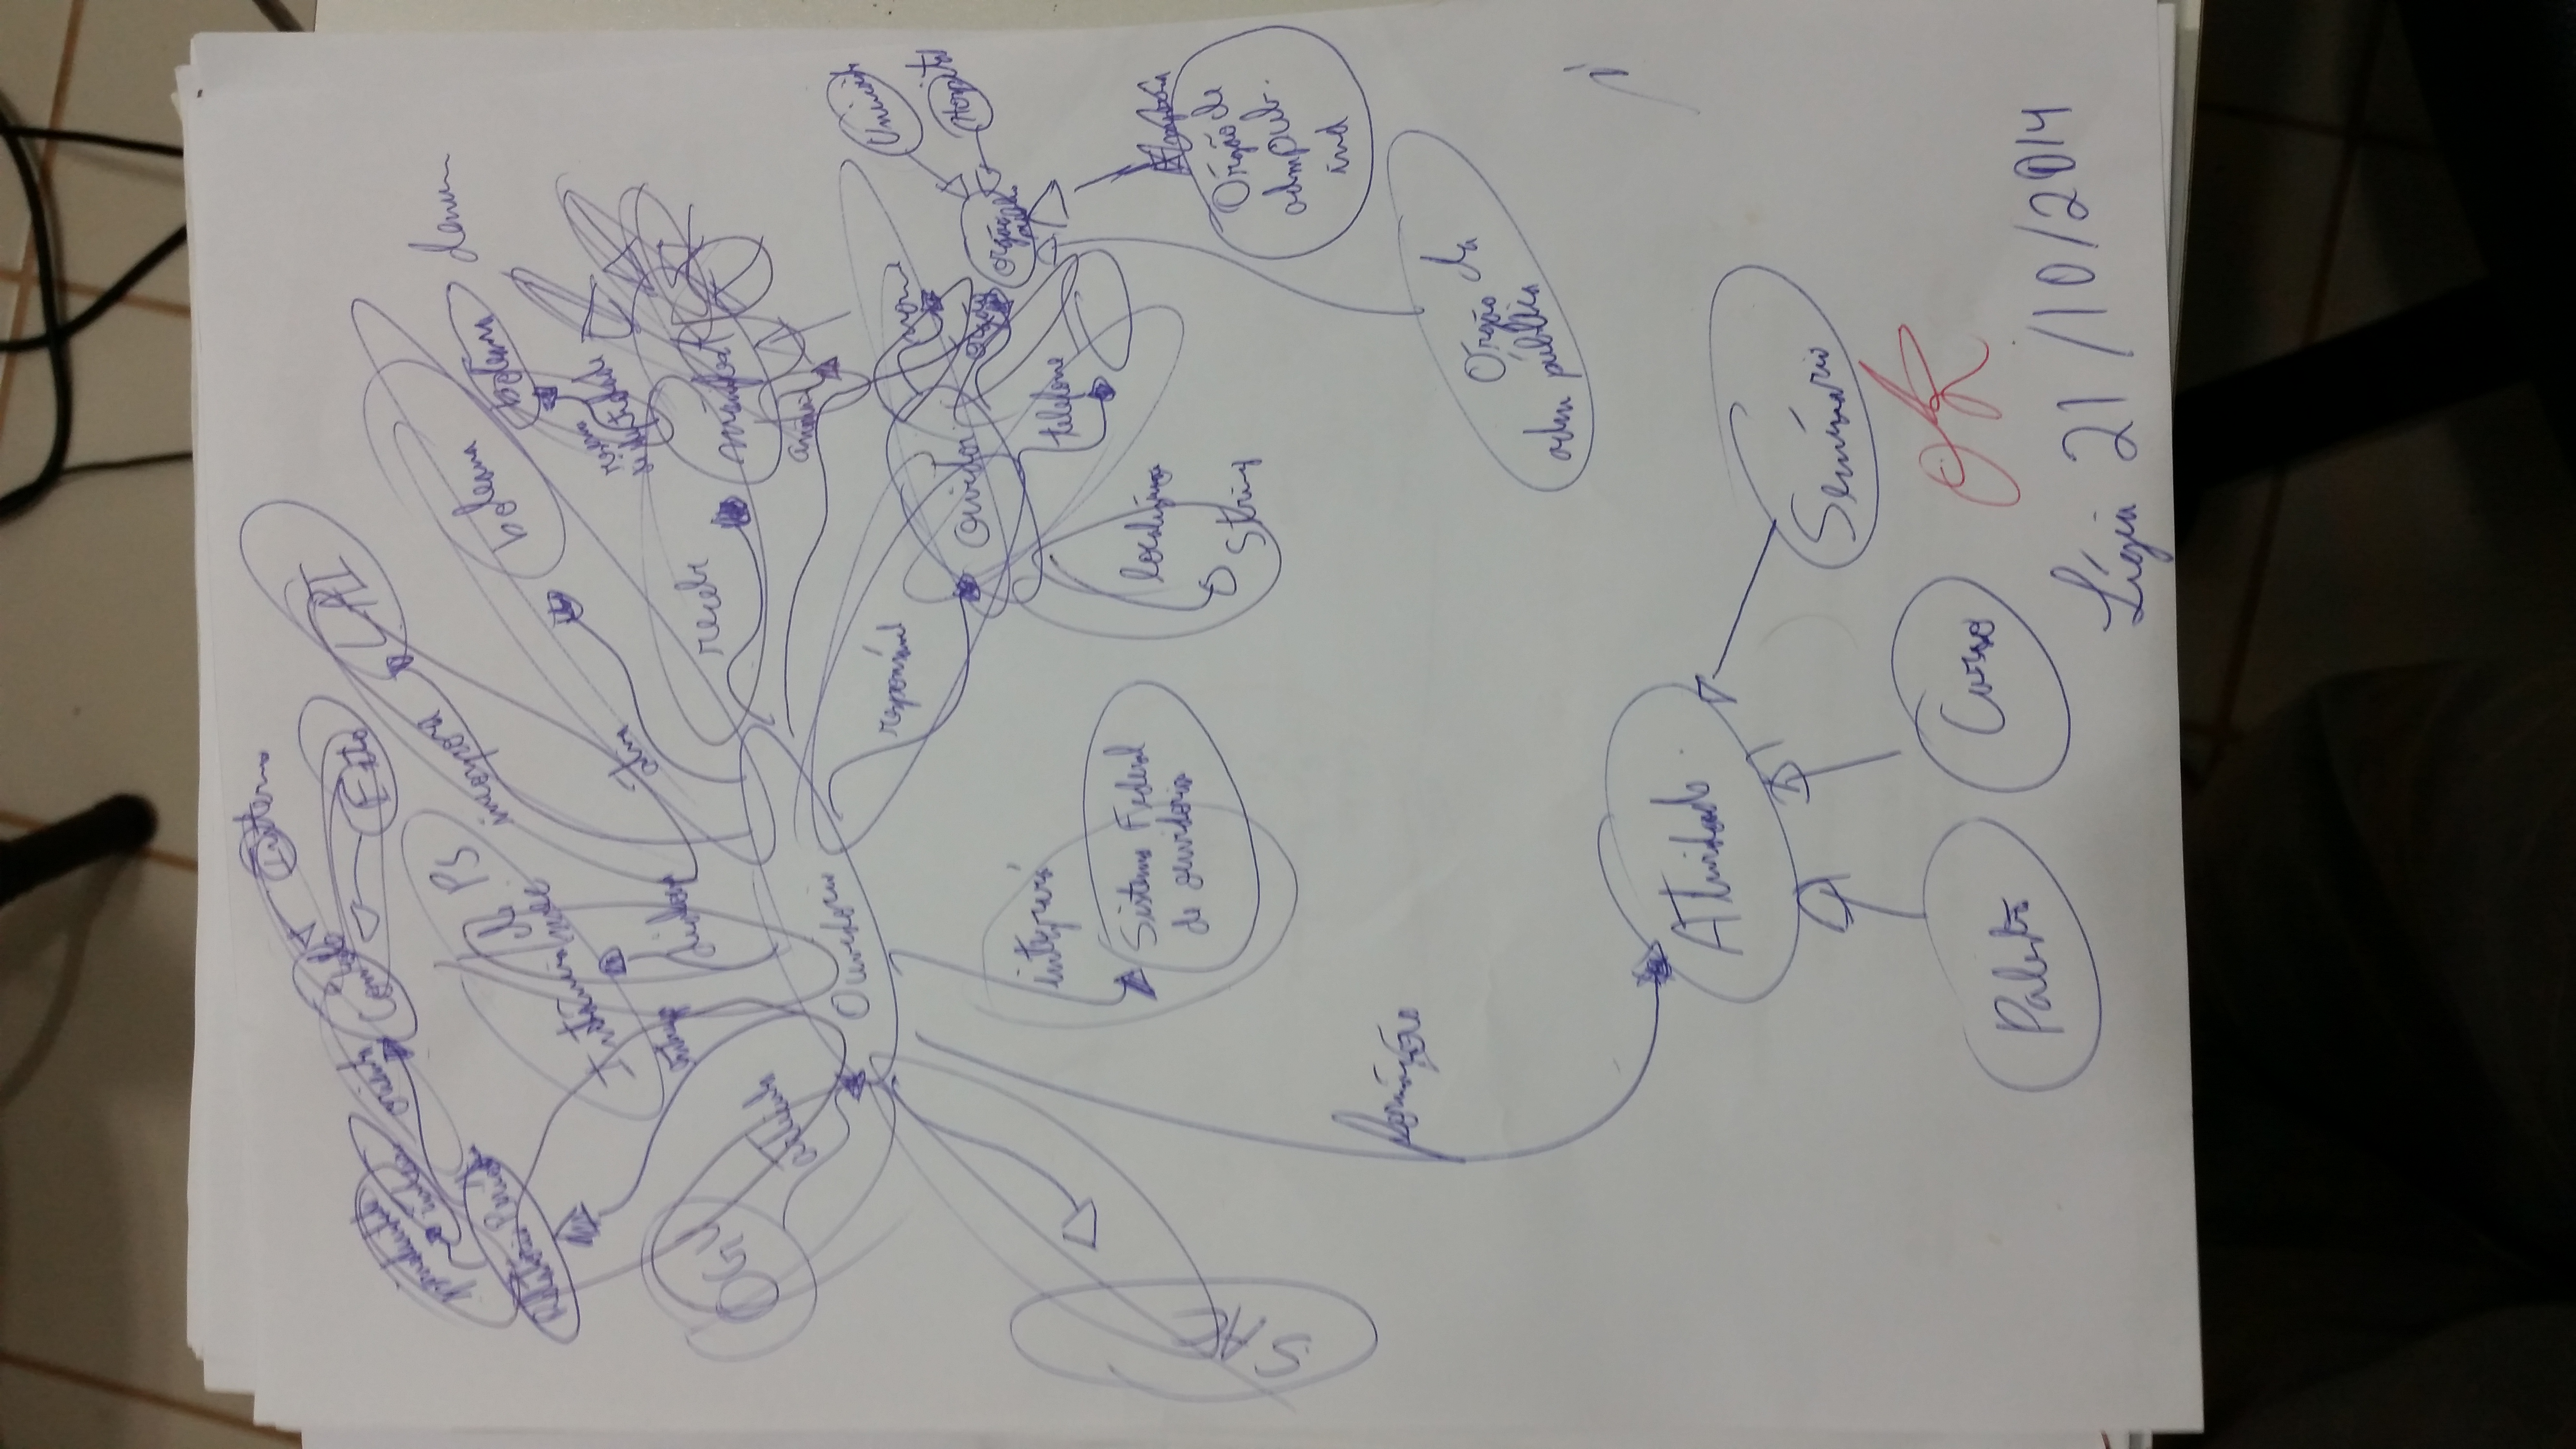
\includegraphics[width=\textwidth,angle=270]{fotos/OuvidoriaLigia.jpg}
  \caption{Diagrama de Ouvidorias desenhado com o acompanhamento de especialista (Lígia).}
\end{figure}
\end{document}
